\chapter{Magnetism, Part 1}
\label{chapter:magnetism1}


%\section{Magnetic Field}

\begin{itemize}
\item Magnetism is generated by moving charged particles, e.g.\ a single
  charge, or an electric current
\item It can also be generated by permanent magnets, or Earth
\item Magnetism affects other \emph{moving} charged particles
\item The vector field is called the \textbf{magnetic field}
\item Magnetic field has unit \textbf{tesla}
\item Magnetic field lines have no ends---they always run in a loop
  \end{itemize}




\section{Magnetic Field Generated by a Moving Point Charge}
\begin{center}
  \pic{.35}{../magnetism/pointchargeB}
\end{center}
A point charge generates an electric field $\bm E$. When it's moving, it
also generates a magnetic field $\bm B$, given by the equation:
\begin{equation}
  \boxed{\bm B=\frac{\mu_0}{4\pi}\frac{q\bm v\times\hat{\bm r}}{r^2}}
\end{equation}
The direction of $\bm B$ can be obtained by applying the
\emph{right-hand rule} if you are not confident with cross products.




%\section{Reminder on the cross product}
%Whenever the ``right-hand rule'' is mentioned, or when an equation has
%``$\sin\theta$'' in it, that usually means that the equation involces a
%cross product in it. Just a reminder on a few properties:
%\begin{itemize}
%\item If $\bm C=\bm A\times\bm B$, then $\bm C$ is perpendicular to both
%  $\bm A$ and $\bm B$.
%\item The length of the cross product of two vectors is:
%  \begin{equation}
%    |\bm A\times\bm B|=|\bm A||\bm B|\sin\theta
%  \end{equation}
%  where $\theta$ is the angle between $\bm A$ and $\bm B$
%\item Cross products are anti-commutable:
%  \begin{equation}
%    \bm A\times\bm B=-\bm B\times\bm A
%  \end{equation}
%\end{itemize}




\section{Magnetic Field Generated by a Moving Point Charge}
\begin{equation}
  \boxed{
    \bm B=\frac{\mu_0}{4\pi}\frac{q\bm v\times\hat r}{r^2}
  }
\end{equation}
\begin{center}
  \begin{tabular}{l|c|c}
    \rowcolor{pink}
    \textbf{Quantity} & \textbf{Symbol} & \textbf{SI Unit} \\ \hline
    Magnetic field                  & $\bm B$ & \si\tesla \\
    Charge                          & $q$      & \si\coulomb \\
    Velocity of the charge          & $\bm v$ & \si{\meter\per\second}\\
    Distance from the moving charge & $r$      & \si\metre\\
    Radial outward unit vector from the charge & $\hat r$ & no units\\
    Permeability of free space & $\mu_0$ & \si{\tesla\metre\per\ampere}
  \end{tabular}
\end{center}
\textbf{Permeability of free space} (or \textbf{vacuum permeability}) is a
constant with a value of
$\mu_0=4\pi\times\num{e-7}\;\si{\tesla\metre\per\ampere}$. It measures how
well a space can become magnetized.




\section{Biot-Savart Law}
  
\pic{.4}{../magnetism/bsav}

An electric current is really many charges particles moving along a wire;
each charge creating its own magnetic field.
The total magnetic field in the wire is the integral of the contribution
($\dl\bm B$) of the current ($I$) from each infinitesimal sections
($\dl\bm L$) of the wire, given by the \textbf{Biot-Savart law}:

\begin{equation}
  \boxed{
    \dl\bm B=\frac{\mu_0}{4\pi}\frac{I\dl\bm L\times\hat r}{r^2}
  }
\end{equation}
The magnetic field in the diagram goes \emph{into} the page
  



\section{Magnetic Field Generated By an Infinitely Long Wire}
  
\pic{.25}{../magnetism/magcur2}

Integrating Biot-Savart law for a point at radial distance $r$ from an
\emph{infinitely-long wire} gives a simple expression:

\begin{equation}
  \boxed{\bm B=\frac{\mu_0(\bm I\times\hat r)}{2\pi r}}
  \quad\text{or}\quad
  \boxed{B=\frac{\mu_0I}{2\pi r}}
\end{equation}

The magnitude and direction current ``vector'' $\bm I$ is straightforward

\begin{tabular}{l|c|c}
  \rowcolor{pink}
  \textbf{Quantity} & \textbf{Symbol} & \textbf{SI Unit} \\ \hline
  Magnetic field      & $\bm B$ & \si\tesla \\
  Current             & $\bm I$ & \si\ampere \\
  Radial direction from the wire & $\hat r$ & (no units)\\
  Radial distance from the wire  & $r$      & \si\metre
\end{tabular}
  



\section{Current-Carrying Wire Loop}
  
\pic{.4}{../magnetism/curloo}

When we shape the current-carrying wire into a loop, we can (again) use
the Biot-Savart law to find the magnetic field away from it.

One loop isn't very interesting (except when you're integrating Biot-Savart
law) but what if we have many loops
  




\section{Wounding Wires Into a Coil}
\begin{itemize}
\item A \textbf{solenoid} is when you wound a wire into a coil
\item You create a magnet very similar to a bar magnet, with an effective
  north pole and a south pole
\item Magnetic field inside the solenoid is uniform
\item Magnetic field strength can be increased by the addition of an iron core
\end{itemize}
\begin{center}
  \pic{.5}{../magnetism/barsol}
\end{center}




\section{A Practical Solenoid}
A practical solenoid usually has hundreds or thousands of turns:
\begin{center}
  \pic{.45}{../magnetism/1020201515330450255}
\end{center}

\vspace{-.2in}
This ``air core'' coil is used for high school and university experiments. It
has approximately 600 turns of copper wire wound around a plastic core.




\section{Magnetic Field Inside a Solenoid}
  
\pic{.4}{../magnetism/magneticfield4}

The magnetic field \textbf{inside} a solenoid is uniform, with its strength
given by:

\begin{equation}
  \boxed{B=\frac{\mu NI}{\ell}}
\end{equation}
    
Direction of $\bm B$ determined by \textbf{right-hand rule}
\begin{center}
  \begin{tabular}{l|c|c}
    \rowcolor{pink}
    \textbf{Quantity} & \textbf{Symbol} & \textbf{SI Unit} \\ \hline
    Magnetic field intensity & $B$    & \si\tesla \\
    Number of coils          & $N$    & \\
    Length of the solenoid   & $\ell$ & \si\metre \\
    Current                  & $I$    & \si\ampere \\
    Effective permeability   & $\mu$  & \si{\tesla.\metre\per\ampere}
  \end{tabular}
\end{center}
  



\section{Permanent Magnets}
Permanent magnets is also based on the motion of charges. This is the
``non-technical'' version\ldots
\begin{enumerate}

\item Electrons inside an atom \emph{spin}. A spinning electron therefore has
  an angular momentum, and generates its own tiny magnetic field.
  \begin{center}
    \pic{.3}{../magnetism/Electron-spin}
    \end{center}
  However, in most full ``shells'', the spin of these electrons are paired,
  so the magnetic fields cancel each other.

\item The orbits of electrons are not always filled, therefore some atoms do
  create some (very small) magnetic field.
  \begin{center}
    \pic{.4}{../magnetism/paramagnetic}
  \end{center}
  The atoms that have unpaired electrons are called \textbf{paramagnetic}
  because they are attracted to magnets; atoms that have no unpaired
  electrons are called \textbf{diamagnetic}.

\item While many atoms exhibit paramagnetism, they do not make good magnets,
  because the atoms are most often arranged in a way where the magnetic fields
  cancel. This is callled \textbf{ferrimagnetism}:
  \begin{center}
    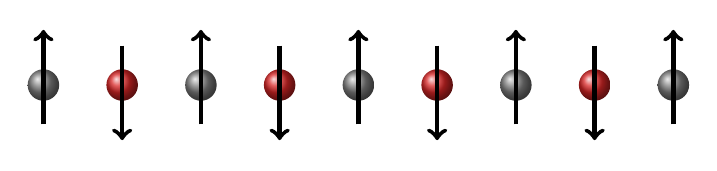
\begin{tikzpicture}
      \foreach\x in {0,2,...,8}{
        \shade[ball color=gray] (\x,0) circle (.2);
        \draw[ultra thick,->] (\x,-.5)--(\x,.7);
      }
      \foreach\x in {1,3,5,7}{
        \shade[ball color=red!70!gray] (\x,0) circle (.2);
        \draw[ultra thick,->] (\x,.5)--(\x,-.7);
      }
      
    \end{tikzpicture}\\
    Ferrimagnetic
  \end{center}
  When they do not cancel, then they can become magnets. This is called
  \textbf{ferromagnetism}:
  \begin{center}
    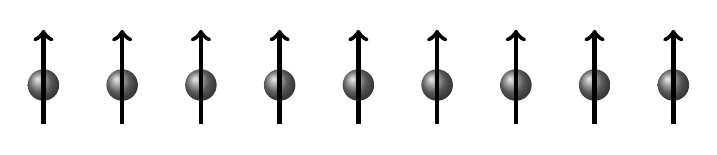
\begin{tikzpicture}
      \foreach\x in {0,1,...,8}{
        \shade[ball color=gray] (\x,0) circle (.2);% node[below right]{$m$};
        \draw[ultra thick,->] (\x,-.5)--(\x,.7);
      }
    \end{tikzpicture}\\
    Ferromagnetic
  \end{center}
  Transitional elements such as iron, nickel and cobalt, and their alloys
  will exhibit ferromagnetism.
  
\item The atoms in these ferromagnetic materials are arranged in ``domains''
  wher their magnetic moment is aligned. In the presence of a strong
  external magnetic field, these domains will line up, creating a magnet.
  \begin{center}
    \pic{.6}{../magnetism/domain}
  \end{center}
\end{enumerate}




\section{Earth}
Earth is also a ``permanent'' magnet, with the \emph{magnetic south pole}
located near the geographic north pole, and the \emph{magnetic north pole}
located near the geographic south pole. The poles are tilted by
$\approx\ang{11}$ from the spin axis.
\begin{center}
  \pic{.5}{../magnetism/mearthbar}
\end{center}
The exact nature of Earth's magnetic field is not known, although it may be
related to ``generator effect'' from Earth's rotation, circulating the
outer-core fluid around.




\section{Amp\`{e}re's Law}

\begin{figure}[ht]
  \centering
  \pic{.4}{../magnetism/amlaw}
\end{figure}

Like Gauss's law is used to calculate electric fields,
\textbf{Amp\`{e}re's law} is used to calculate the magnetic field for
symmetric configurations:

\begin{equation}
  \boxed{\oint_C \bm B\cdot\dl\bm\ell=\mu_0 I_C}
\end{equation}
where
\begin{itemize}
\item $C$ is a closed curve around a current (``Amperian loop'')
\item $\dl\bm\ell$ is an infinitesimal length along the closed curve
\item $I_c$ is the net current that penetrates the area bounded by $C$
\end{itemize}
  




\section{Application of Amp\`{e}re's Law: Infinitely-Long Wire}

\begin{figure}[ht]
  \centering
  \pic{.4}{../magnetism/4iM3O}
\end{figure}

An \emph{infinitely} long wire must generate a magnetic field that only
depend on radial distance. We place an Amperian loop as a circle of radius
$r$ inside the toroid. Amp\`{e}re's law reduces to:
\begin{equation}
  \oint_C \bm B\cdot\dl\bm\ell=\mu_0 I_C
  \;\rightarrow\;
  B(2\pi r)=\mu_0 I
\end{equation}
From this, we get our expression of the magnetic field from an infinitely
long wire:
\begin{equation}
  B=\frac{\mu_0 I}{2\pi r}
\end{equation}
  




\section{Toroid}
\begin{figure}[ht]
  \centering  
  \pic{.4}{../magnetism/toroid}
\end{figure}

{\scriptsize A toroid consists of a current-\\
  carrying wire wound around a donut-shaped core \par}

Another application of Amp\`{e}re's law is the \textbf{toroid}. This time,
we put our loop at $a<r<b$ inside the toroid. Once again, because of
symmetry, Amp\`{e}re's law reduces to:

\begin{align*}
  \oint_C \bm B\cdot\dl\bm\ell &=\mu_0 I_C\\
  B(2\pi r)&=\mu_0 NI\\
  B&=\frac{\mu_0 NI}{2\pi r}
\end{align*}
where $N$ is the number of times the wire is wound around the core
  



When the loop is placed at $r<a$, there is no enclosed
current, and therefore the magnetic field is zero:
\begin{equation}
  B=0\quad\text{for}\quad r<a
\end{equation}
When the loop is placed at $r>b$, the amount of current
penetrating the loop is the same in both direction, i.e.\ $I_c=0$, and
\begin{equation}
  B=0\quad\text{for}\quad r>b
\end{equation}
    
In fact, magnetic field \emph{only} exists inside the core, between $a$ and
$b$.
  





\section{Magnetic Force}

  
\begin{center}
  Gravitational Field $\bm g$
\end{center}
\begin{itemize}
\item Generated by massive objects
\item Affects massive objects
\end{itemize}

\begin{center}
  Electric Field $\bm E$
\end{center}
\begin{itemize}
\item Generated by charged particles
\item Affects charged particles
\end{itemize}

\begin{center}
  Magnetic Field $\bm B$
\end{center}
\begin{itemize}
\item Generated by \emph{moving} charged particles
\item Affects moving charged particles
\end{itemize}
  




\section{Lorentz Force Law}
Since a moving charge or current create both electric and magnetic fields,
another moving charge is therefore affected by both $\bm E$ and $\bm B$.
The total effect is given by the \textbf{Lorentz force law}:
\begin{equation}
  \boxed{\bm F=q(\bm E+\bm v\times\bm B)}
\end{equation}
$\bm F_q=q\bm E$ is the electrostatic force, and
$\bm F_m=q\bm v\times\bm B$ is the magnetic force.
\begin{center}
  \begin{tabular}{l|c|c}
    \rowcolor{pink}
    \textbf{Quantity} & \textbf{Symbol} & \textbf{SI Unit} \\ \hline
    Total force on the moving charge & $\bm F$ & \si\newton \\
    Charge                 & $q$      & \si\coulomb \\
    Velocity of the charge & $\bm v$ & \si{\metre\per\second} \\
    Magnetic field         & $\bm B$ & \si\tesla \\
    Electric field         & $\bm E$ & \si{\newton\per\coulomb}
  \end{tabular}
\end{center}




\section{Magnetic Force on a Current-Carrying Conductor}
Likewise, $\bm B$ exerts a force on another current-carrying conductor.
\begin{equation}
  \boxed{\dl F_m=\bm I\dl\ell\times\bm B}
\end{equation}
\begin{center}
  \begin{tabular}{l|c|c}
    \rowcolor{pink}
    \textbf{Quantity} & \textbf{Symbol} & \textbf{SI Unit} \\ \hline
    Magnetic force on the conductor   & $\bm F_m$ & \si\newton \\
    Electric current in the conductor & $\bm I$   & \si\ampere \\
    Length of the conductor           & $\ell$     & \si\metre \\
    Magnetic field                    & $\bm B$   & \si\tesla
  \end{tabular}
\end{center}




\section{Magnetic Force on Two Current-Carrying Wires}
\begin{figure}[ht]
  \centering
  \pic{.4}{../magnetism/wirefor}
\end{figure}

Two parallel current-carrying wires of length $L$ are at a distance $r$
apart. Magnetic field at wire $2$ from current $I_1$ has constant strength
along the wire, given by:
    
\begin{equation}
  B=\frac{\mu_0I_1}{2\pi r}
\end{equation}

The force of $B$ on $I_2$ is:

\begin{equation}
  F=I_2LB=\frac{\mu_0I_1I_2L}{2\pi r}
  \;\rightarrow\;
  \boxed{\frac FL=\frac{\mu_0I_1I_2}{2\pi r}}
\end{equation}
$I_1$ also exerts the same force on $I_2$, pulling the wires toward each
other. (We should expect this because of third law of motion.)
  




\section{Circular Motion Caused by a Magnetic Field}
When a charged particle enters a magnetic field at right angle\ldots
\begin{itemize}
\item Magnetic force $\bm F_m$ perpendicular to both velocity $\bm v$ and
  magnetic field $\bm B$.
\item Results in circular motion
\end{itemize}
Centripetal force $\bm F_c$ is provided by the magnetic force $\bm F_m$.
Equating the two expressions:

\begin{equation}
  \frac{mv^2}r=qvB
\end{equation}
  
We can solve for $r$ get the radius for a charge with a known
mass, or solve for mass $m$ of a charged particle based on its radius:  

\begin{equation}
  r = \frac{mv}{qB}\quad\quad\quad m=\frac{qrB}v
\end{equation}

